% ============================================================
% COLINHA DO TCC — Explicação Completa em Linguagem Simples
% Lucas Fiori Magalhães Machado — 29/04/2026
% ============================================================
\documentclass[12pt,a4paper]{article}
\usepackage[utf8]{inputenc}
\usepackage[T1]{fontenc}
\usepackage[brazil]{babel}
\usepackage[top=2.5cm,bottom=2.5cm,left=2.5cm,right=2.5cm]{geometry}
\usepackage{amsmath}
\usepackage{graphicx}
\usepackage{xcolor}
\usepackage{booktabs}
\usepackage{array}
\usepackage{enumitem}
\usepackage{fancyhdr}

% ---------- Cabeçalho / Rodapé ----------
\pagestyle{fancy}
\fancyhf{}
\rhead{\small\textcolor{gray}{Colinha do TCC --- Lucas Fiori Magalhães Machado}}
\cfoot{\thepage}
\renewcommand{\headrulewidth}{0.4pt}

% ---------- Cores ----------
\definecolor{azul}{RGB}{0,90,160}
\definecolor{verde}{RGB}{30,130,60}
\definecolor{laranja}{RGB}{200,100,0}
\definecolor{cinza}{RGB}{110,110,110}
\definecolor{roxo}{RGB}{110,0,150}

% ---------- Comandos de destaque ----------
\newcommand{\num}[1]{\textcolor{azul}{\textbf{#1}}}
\newcommand{\ok}[1]{\textcolor{verde}{\textbf{#1}}}
\newcommand{\alerta}[1]{\textcolor{laranja}{\textbf{#1}}}
\newcommand{\term}[1]{\textcolor{roxo}{\textit{#1}}}
\newcommand{\obs}[1]{\par\small\textcolor{cinza}{\textit{Obs.: #1}}\normalsize\par}

% ---------- Espaçamento de parágrafo ----------
\setlength{\parindent}{0pt}
\setlength{\parskip}{9pt plus2pt minus1pt}

% ---------- Listas sem espaço extra ----------
\setlist[itemize]{noitemsep, topsep=4pt}
\setlist[enumerate]{noitemsep, topsep=4pt}
\setlist[description]{noitemsep, topsep=4pt}

% ============================================================
\begin{document}

% -------- CAPA --------
\begin{titlepage}
\centering
\vspace*{2cm}
{\Huge\textbf{Colinha do TCC}}\\[0.7em]
{\Large Explicação Completa em Linguagem Simples}\\[2em]
\rule{\textwidth}{1pt}\\[0.8em]
{\large\itshape
  Detecção Automatizada de Estratégias \textbf{Call2Go}:\\[0.3em]
  Pipeline Cross-Platform para a Indústria Musical Brasileira
}\\[0.8em]
\rule{\textwidth}{1pt}\\[3em]
{\large Lucas Fiori Magalhães Machado}\\[0.4em]
{\normalsize Bacharelado em Ciência da Computação --- PUC Minas}\\[4em]
{\large\textbf{29 de abril de 2026}}
\vfill
{\small
  Este documento é um guia de bolso para entender e explicar o TCC.\\
  Cada número, gráfico e teste estatístico está explicado em linguagem simples.\\[0.5em]
  \textit{Não é o artigo final --- é a sua cola pessoal.}
}
\end{titlepage}

\tableofcontents
\newpage

% ============================================================
\section{O que é esse TCC?}
% ============================================================

O TCC estuda uma prática muito comum na indústria musical brasileira chamada
\term{Call2Go}. Em resumo, a pesquisa faz duas coisas principais:

\begin{enumerate}
  \item \textbf{Cria uma ferramenta automática} capaz de detectar se um artista
        está usando essa estratégia em seus vídeos do YouTube.
  \item \textbf{Testa estatisticamente} se essa estratégia faz diferença real:
        artistas que usam Call2Go ganham mais visualizações? Ficam mais populares
        no Spotify?
\end{enumerate}

O foco central do trabalho \textbf{não} é sobre música, artistas ou o mercado
fonográfico em si. O que realmente importa é: \ok{``a ferramenta que criamos é
confiável?''} Os artistas são apenas o banco de dados utilizado para testar essa
ferramenta.

\textbf{Por que isso importa?} Sem uma ferramenta confiável, qualquer conclusão
sobre Call2Go seria suspeita. Então, antes de analisar qualquer dado, foi
necessário garantir que o detector funcionava corretamente --- e isso foi feito
por meio de uma validação com humanos.

% ============================================================
\section{O que é Call2Go?}
% ============================================================

Imagine que você está assistindo a um clipe no YouTube. Lá na descrição do
vídeo, o artista coloca algo parecido com:

\begin{quote}
  \textit{``Ouça agora no Spotify: https://open.spotify.com/...''} \\
  \textit{``Disponível no Spotify $\downarrow$ bit.ly/MinhaMusica''} \\
  \textit{``Stream agora no Spotify!''}
\end{quote}

Isso é um \term{Call2Go}: uma \textbf{chamada de ação} (\textit{call-to-action})
que leva o ouvinte do YouTube diretamente para o Spotify.

\textbf{Por que os artistas fazem isso?} A lógica é simples: o YouTube é
gratuito, tem alcance enorme e qualquer pessoa pode acessar. Já o Spotify paga
diretamente ao artista por cada \textit{stream}. Então faz sentido usar o YouTube
como vitrine para converter fãs em ouvintes pagos/recorrentes no Spotify.

O Call2Go pode aparecer em dois lugares diferentes:
\begin{itemize}
  \item \textbf{Na descrição do vídeo}: um link ou texto direto no campo de
        descrição do YouTube (o texto que aparece abaixo do vídeo).
  \item \textbf{Na bio do canal}: na aba ``Sobre'' do canal do artista no
        YouTube, onde ele pode colocar links externos para outras plataformas.
\end{itemize}

O TCC verifica os \textbf{dois lugares} e combina as detecções de duas formas:
\begin{itemize}
  \item \textbf{OR}: Call2Go detectado no vídeo \textbf{OU} no canal
        (qualquer um dos dois basta).
  \item \textbf{AND}: Call2Go detectado no vídeo \textbf{E} no canal ao mesmo
        tempo (os dois precisam estar presentes).
\end{itemize}

% ============================================================
\section{De onde vieram os dados?}
% ============================================================

\subsection{Quem foram os artistas?}

Foram selecionados \num{67 artistas brasileiros} que apareceram simultaneamente
nos dois rankings abaixo durante o primeiro trimestre de 2026 (Q1~2026 =
janeiro, fevereiro e março de 2026):

\begin{itemize}
  \item \textbf{Spotify Top 200 Brasil}: ranking das 200 músicas mais ouvidas
        no Spotify Brasil por semana.
  \item \textbf{YouTube Top 100 Brasil}: ranking dos 100 vídeos mais assistidos
        no YouTube Brasil por semana.
\end{itemize}

O critério foi aparecer em pelo menos uma semana das \num{13 semanas} do
Q1~2026 nos \textbf{dois} rankings ao mesmo tempo. Isso é chamado de
\term{persistência cross-platform}: o artista é relevante nas duas plataformas.

A escolha de usar os dois rankings juntos foi proposital: só interessam
artistas que realmente usam as duas plataformas de forma ativa, porque o
estudo compara YouTube com Spotify.

\subsection{Quantos vídeos foram analisados?}

Para cada um dos 67 artistas, foram coletados os \num{30 vídeos mais
visualizados} de cada canal do YouTube. O total ficou em:

\[
  67 \text{ artistas} \times \approx 30 \text{ vídeos} = \num{1.641 vídeos}
\]

\obs{O número não é exatamente 2.010 (67 × 30) porque alguns canais tinham
menos de 30 vídeos disponíveis no momento da coleta.}

\subsection{De onde vieram os dados de cada plataforma?}

\begin{itemize}
  \item \textbf{YouTube} --- via YouTube Data API v3 (ferramenta oficial do
        Google). Foram coletadas as descrições dos vídeos, número de
        visualizações e data de publicação de cada vídeo.
  \item \textbf{Spotify} --- via Spotify Web API (ferramenta oficial do
        Spotify). Coletou-se a \term{popularidade} (índice de 0 a 100 que o
        próprio Spotify calcula com base em recência e frequência de streams) e
        o número de seguidores de cada artista. O snapshot (foto dos dados) foi
        tirado em 22 de abril de 2026.
  \item \textbf{Last.fm} --- via Last.fm API. O Last.fm é uma rede social de
        música que registra automaticamente o que as pessoas ouvem
        (\term{scrobbling}). Foram coletados: ouvintes mensais, scrobbles (total
        de reproduções registradas) e presença nos charts brasileiros do Last.fm.
        Serve como uma \textbf{terceira plataforma independente} para cruzar e
        validar os dados.
  \item \textbf{Scraping dos canais} --- a aba ``Sobre'' de cada canal do
        YouTube tem links externos, mas a API oficial do YouTube \textbf{não
        fornece} esses links. Por isso foi necessário usar um \term{scraper}: um
        programa que acessa a página do canal diretamente, lê o código HTML e
        extrai os links ali presentes.
\end{itemize}

% ============================================================
\section{O pipeline: os 15 passos do processo}
% ============================================================

Um \term{pipeline} é uma sequência de etapas automatizadas, onde a saída de
cada etapa é a entrada da próxima --- como uma linha de produção de fábrica.
O pipeline do TCC tem \num{15 etapas} no total, roda do início ao fim em
aproximadamente \num{40 segundos} e gera \num{30 artefatos} verificáveis
(arquivos de saída auditáveis).

\bigskip
\noindent\textbf{\textcolor{azul}{Bloco 1 — Coleta de Dados (Etapas 1--5)}}

\begin{description}[leftmargin=1.8em, style=nextline]
  \item[Etapa 1 --- Lista de artistas]
    Lê um arquivo CSV com os 67 artistas selecionados manualmente dos charts e
    os cadastra no sistema como ponto de partida de tudo.
  \item[Etapa 2 --- Coleta YouTube]
    Para cada artista, acessa o canal do YouTube via API e baixa os dados dos
    30 vídeos mais visualizados: título, descrição completa, número de
    visualizações e data de publicação.
  \item[Etapa 3 --- Coleta Spotify]
    Para cada artista, consulta a API do Spotify e salva dois valores:
    popularidade (0--100) e número de seguidores.
  \item[Etapa 4 --- Coleta Last.fm]
    Para cada artista, consulta a API do Last.fm e salva: ouvintes mensais,
    total de scrobbles e se o artista está nos charts brasileiros do Last.fm.
  \item[Etapa 5 --- Scraping de canais]
    Acessa a aba ``Sobre'' de cada canal do YouTube via scraper e extrai os
    links externos ali listados (por exemplo, link do Spotify na bio do canal).
\end{description}

\bigskip
\noindent\textbf{\textcolor{verde}{Bloco 2 — Detecção e Banco de Dados (Etapas 6--7)}}

\begin{description}[leftmargin=1.8em, style=nextline]
  \item[Etapa 6 --- Detecção Call2Go]
    Aplica o motor de detecção (explicado na Seção~\ref{sec:detector}) sobre
    as descrições dos vídeos e sobre os links dos canais. Gera para cada
    vídeo: detectou no vídeo? detectou no canal? resultado OR? resultado AND?
  \item[Etapa 7 --- Data Warehouse]
    Salva todos os dados coletados e as detecções em um banco de dados SQLite
    com \num{6 tabelas} organizadas em \term{star schema} (formato padrão para
    análises de dados, com uma tabela central e tabelas de apoio ao redor).
\end{description}

\bigskip
\noindent\textbf{\textcolor{verde}{Bloco 3 — Análises Estatísticas (Etapas 8--12)}}

\begin{description}[leftmargin=1.8em, style=nextline]
  \item[Etapa 8 --- EDA (Análise Exploratória)]
    Visão geral dos dados: distribuições, médias, boxplots. É a etapa de
    ``olhar os dados'' antes de qualquer teste formal.
  \item[Etapa 9 --- Mann-Whitney]
    Testa as hipóteses H2 e H3: Call2Go afeta visualizações no YouTube? Afeta
    popularidade no Spotify?
  \item[Etapa 10 --- Cross-Platform]
    Analisa a relação estatística entre as métricas do YouTube e do Spotify
    por artista.
  \item[Etapa 11 --- Last.fm Bridge]
    Cruza os dados do Last.fm com YouTube e Spotify, usando o Last.fm como
    terceira fonte independente.
  \item[Etapa 12 --- Validação Bidirecional]
    Analisa a correlação nos dois sentidos: YouTube$\to$Spotify e
    Spotify$\to$YouTube. Qual plataforma influencia a outra?
\end{description}

\bigskip
\noindent\textbf{\textcolor{verde}{Bloco 4 — Análise Temporal (Etapas 13--15)}}

\begin{description}[leftmargin=1.8em, style=nextline]
  \item[Etapa 13 --- Datas Spotify]
    Recupera quando cada artista apareceu pela primeira vez nos charts do
    Spotify, para poder calcular a diferença de tempo em relação ao YouTube.
  \item[Etapa 14 --- Ranking Fusion]
    Cria um score combinado cruzando as posições dos artistas nos rankings de
    YouTube, Spotify e Last.fm simultaneamente.
  \item[Etapa 15 --- Análise Temporal]
    Calcula a defasagem de tempo (lag) entre a atividade no YouTube e a
    entrada nos charts do Spotify, e testa se essa defasagem é correlacionada
    com o desempenho nos charts.
\end{description}

\bigskip
\noindent\textbf{\textcolor{roxo}{Etapa adicional --- Validação Independente}}

Fora do pipeline automatizado, foi feita uma validação manual com \num{91
vídeos adversariais} (casos propositalmente difíceis de classificar). Um
humano analisou cada vídeo \textbf{sem saber} o que o detector tinha
classificado (\term{anotação às cegas} = sem viés de confirmação). As
respostas do humano foram comparadas com as do detector para medir a
confiabilidade.

% ============================================================
\section{Como o detector funciona?}
\label{sec:detector}
% ============================================================

O detector é um sistema de \term{busca de texto inteligente} baseado em
\term{regex} (\textit{expressões regulares}). Pense num regex como uma
pesquisa avançada --- tipo o Ctrl+F do Word, mas com regras muito mais
sofisticadas que entendem padrões, variações e contexto.

\subsection{Dois níveis de detecção}

O detector opera em \textbf{dois lugares independentes} em paralelo:

\begin{itemize}
  \item \textbf{Nível Vídeo}: analisa a \textbf{descrição de cada vídeo} do
        YouTube (o texto que aparece abaixo do vídeo).
  \item \textbf{Nível Canal}: analisa os \textbf{links externos} listados na
        aba ``Sobre'' do canal e também a bio do canal.
\end{itemize}

\subsection{As 4 regras de busca no nível vídeo}

Dentro da descrição de cada vídeo, o sistema procura 4 tipos de padrões:

\begin{description}[leftmargin=1.8em]
  \item[Regra R1 --- Links diretos do Spotify]
    Procura pelos domínios \texttt{open.spotify.com}, \texttt{spoti.fi} ou
    \texttt{sptfy.com} no texto. Se encontrar qualquer um desses, é Call2Go.
    Exemplo: \textit{``https://open.spotify.com/album/abc123''}.

  \item[Regra R2 --- Links curtos com rótulo ``Spotify'']
    Procura por links encurtados (\texttt{bit.ly}, \texttt{lnk.to}, etc.)
    que estejam a menos de 50 caracteres da palavra ``spotify'' no texto.
    Exemplo: \textit{``Spotify: bit.ly/MinhaFaixa''} --- o ``bit.ly'' e o
    ``Spotify'' estão próximos, então é Call2Go.

  \item[Regra R3 --- Token ``Spotify'' na própria URL]
    Procura por URLs que tenham a palavra \textit{spotify} ou \textit{sptfy}
    dentro do próprio endereço (ex: \textit{``linkr.to/spotify-artista''}).

  \item[Regra R4 --- Chamadas verbais sem link]
    Procura por frases em português como \textit{``ouça no Spotify''},
    \textit{``disponível no Spotify''} ou \textit{``stream agora no
    Spotify''} --- mesmo sem nenhum link. Captura a intenção de direcionar o
    ouvinte mesmo quando o artista só escreveu o texto sem colocar URL.
\end{description}

\subsection{Filtro anti-falsos-positivos}

Antes de aplicar qualquer regra, o texto passa por um \textbf{filtro} que
descarta frases que mencionam o Spotify sem intenção de direcionar o ouvinte.
Exemplos de frases que seriam \textbf{ignoradas}:

\begin{itemize}
  \item \textit{``\#1 no Spotify Brasil''} (apenas falando sobre uma posição
        em ranking)
  \item \textit{``500 milhões de plays no Spotify''} (apenas mostrando
        estatística)
\end{itemize}

Sem esse filtro, esses casos seriam detectados erroneamente como Call2Go.

\subsection{Lógica OR e AND}

O sistema combina os resultados dos dois níveis de duas formas:

\begin{itemize}
  \item \textbf{OR (métrica primária)}: o vídeo é marcado como Call2Go se
        \textbf{o vídeo OU o canal} tiver Call2Go. Basta um dos dois ter.
        Captura qualquer uso da estratégia, mesmo que parcial.
  \item \textbf{AND (métrica secundária)}: o vídeo é marcado como Call2Go
        somente se \textbf{o vídeo E o canal} tiverem Call2Go ao mesmo tempo.
        Captura a forma mais completa e intencional da estratégia.
\end{itemize}

% ============================================================
\section{O que o detector encontrou: as detecções}
% ============================================================

Após rodar o detector sobre os 1.641 vídeos, estes foram os resultados:

\medskip
\begin{center}
\begin{tabular}{lrr}
\toprule
\textbf{Nível / Métrica} & \textbf{Vídeos} & \textbf{\%} \\
\midrule
Detecção no vídeo (descrição) & 196 & 11,9\% \\
Detecção no canal (bio/links) & 410 & 25,0\% \\
\midrule
\textbf{OR --- vídeo OU canal (métrica principal)} & \textbf{518} & \textbf{31,6\%} \\
AND --- vídeo E canal simultaneamente           & 88  & 5,4\%  \\
Sem Call2Go (OR)                                & 1.123 & 68,4\% \\
\midrule
\textbf{Total}                                  & \textbf{1.641} & \textbf{100\%} \\
\bottomrule
\end{tabular}
\end{center}
\medskip

\textbf{Como interpretar cada linha:}

\begin{itemize}
  \item \num{196 vídeos (11,9\%)} tinham Call2Go detectado \textbf{apenas na
        descrição do vídeo} --- o artista colocou o link ou a chamada na
        descrição de cada vídeo individualmente.
  \item \num{410 vídeos (25,0\%)} tinham Call2Go detectado \textbf{pelo canal}
        --- significa que o canal do artista tem link do Spotify na aba
        ``Sobre'', e todos os vídeos desse canal herdam essa detecção.
  \item \num{518 vídeos (31,6\%)} têm Call2Go no sentido OR: quase \textbf{1
        em cada 3 vídeos} do corpus tem alguma forma da estratégia. Esta é a
        métrica principal.
  \item \num{88 vídeos (5,4\%)} têm AND: o artista colocou Call2Go nos
        \textbf{dois lugares} ao mesmo tempo. É a forma mais intencional e
        completa da estratégia.
  \item \num{1.123 vídeos (68,4\%)} \textbf{não} têm Call2Go em lugar nenhum.
\end{itemize}

\textbf{Observação importante:} o canal é a fonte dominante de detecção
(25\%) comparado ao vídeo (11,9\%). Isso faz sentido: é muito mais prático
para o artista colocar o link de Spotify uma vez na bio do canal do que
escrever em cada vídeo individualmente.

% ============================================================
\section{O Boxplot: comparando visualizações}
% ============================================================

\begin{figure}[h!]
\centering
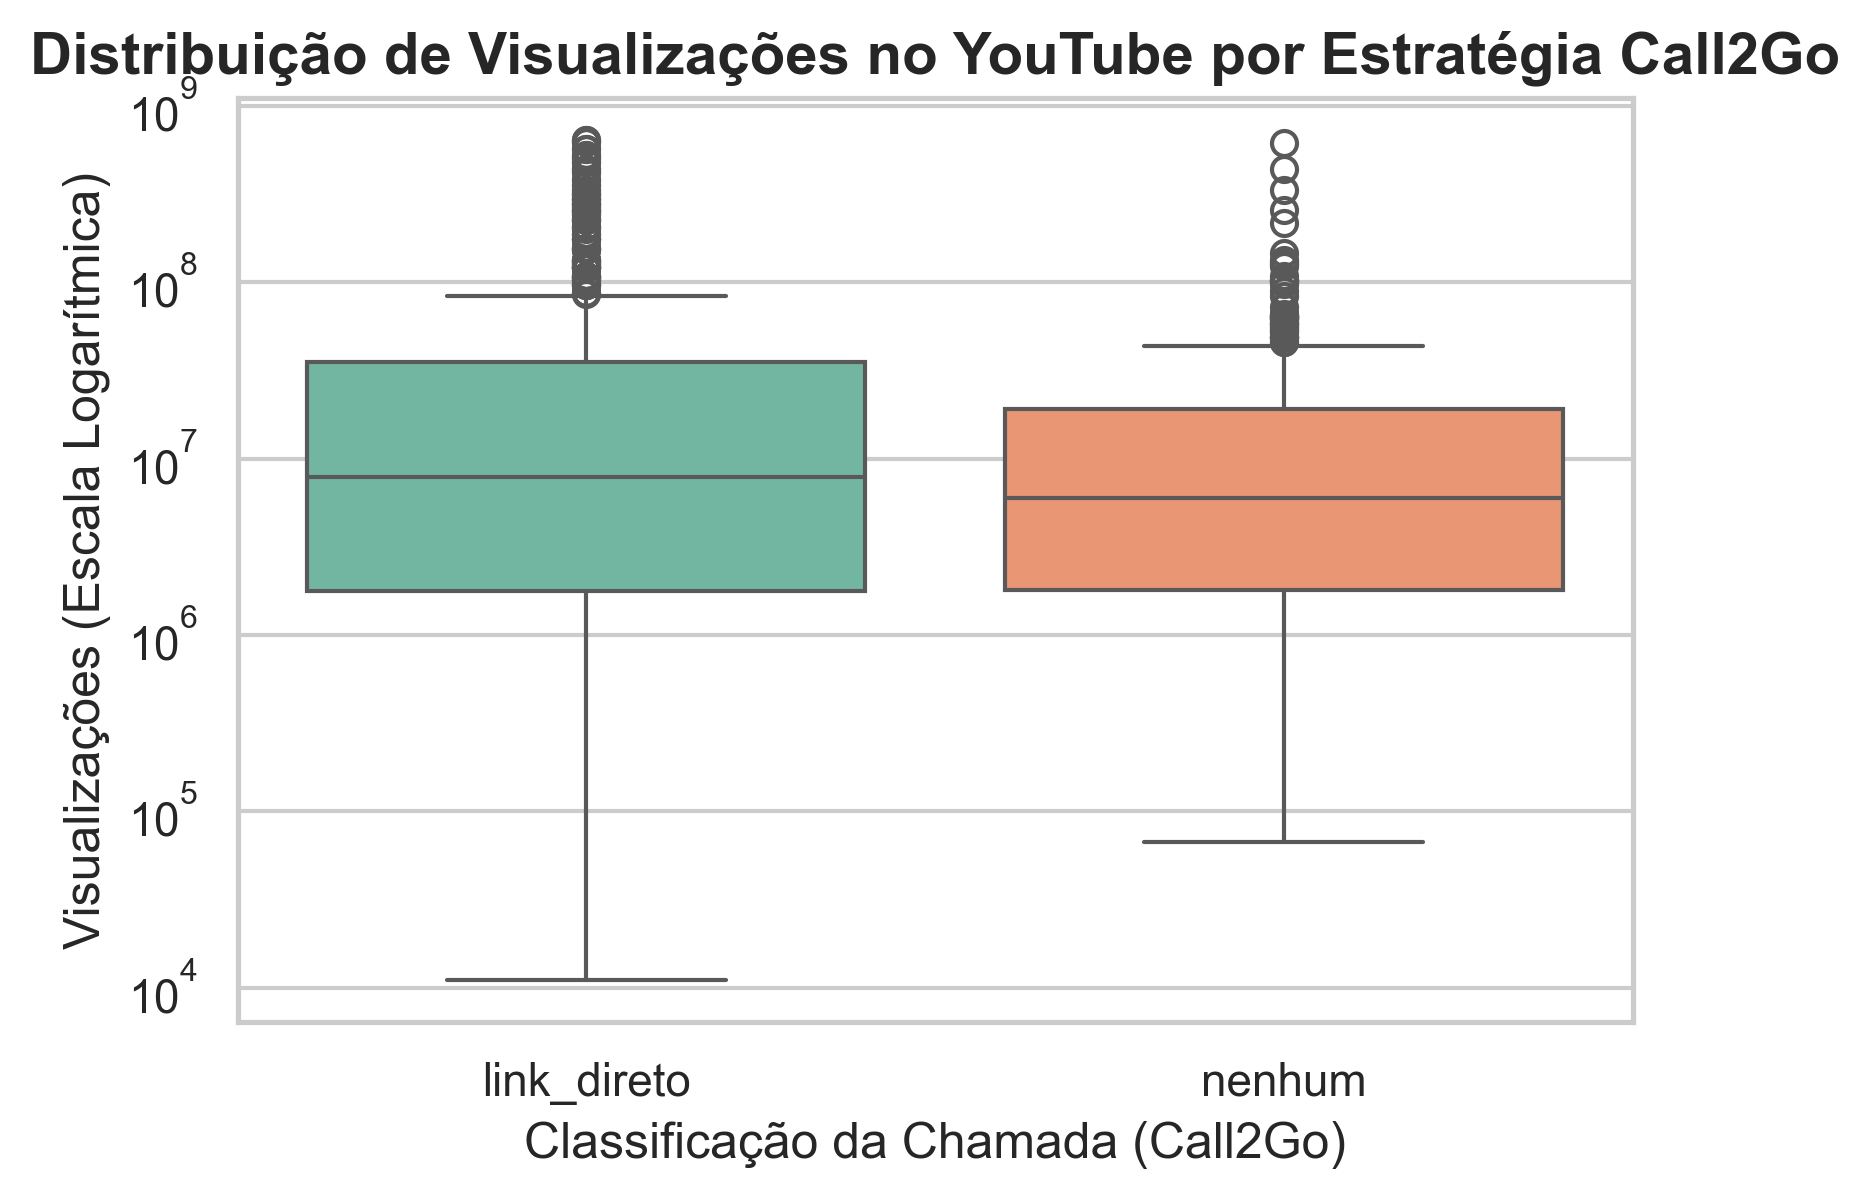
\includegraphics[width=0.90\textwidth]{../artigo_latex/figs/boxplot_call2go_views.png}
\caption{Boxplot comparativo de visualizações (escala log) entre vídeos
  \textbf{com} Call2Go OR ($n=518$) e \textbf{sem} Call2Go ($n=1.123$).}
\label{fig:boxplot}
\end{figure}

\subsection{O que é um boxplot?}

Um boxplot é um gráfico que resume como os valores estão distribuídos num
grupo. Cada elemento do gráfico tem um significado:

\begin{itemize}
  \item \textbf{A caixa (retângulo)}: representa onde ficam os 50\% do meio
        dos dados. A borda de baixo é o 25\textordmasculine{} percentil; a
        borda de cima é o 75\textordmasculine{} percentil.
  \item \textbf{A linha dentro da caixa}: é a \textbf{mediana} --- o valor
        central (metade dos dados fica acima, metade abaixo).
  \item \textbf{Os ``fios'' (whiskers)}: estendem até os valores mais extremos
        que ainda são considerados normais.
  \item \textbf{Os pontos fora dos fios}: são outliers (valores atípicos muito
        acima ou abaixo da maioria).
\end{itemize}

\subsection{O que o gráfico da Figura~\ref{fig:boxplot} mostra?}

O gráfico compara dois grupos lado a lado:

\begin{itemize}
  \item \textbf{Grupo esquerdo}: vídeos \textbf{com} Call2Go OR (518 vídeos)
  \item \textbf{Grupo direito}: vídeos \textbf{sem} Call2Go (1.123 vídeos)
\end{itemize}

O eixo Y (vertical) está em \textbf{escala logarítmica}: cada traço
representa 10 vezes mais visualizações que o anterior. Isso é necessário
porque as visualizações variam enormemente (de alguns milhares até centenas
de milhões).

\textbf{Conclusão visual:} As duas caixas estão quase na mesma altura. As
medianas dos dois grupos são muito próximas. Isso já mostrava visualmente
que vídeos com e sem Call2Go têm basicamente o mesmo desempenho em
visualizações. Os testes estatísticos da próxima seção confirmaram isso
formalmente.

% ============================================================
\section{Testes estatísticos: hipóteses H2 e H3}
% ============================================================

\subsection{O que são H2 e H3?}

\begin{itemize}
  \item \textbf{H2}: Vídeos com Call2Go têm \textbf{mais visualizações} no
        YouTube do que vídeos sem Call2Go?
  \item \textbf{H3}: Artistas com mais Call2Go têm \textbf{maior popularidade}
        no Spotify?
\end{itemize}

\subsection{O que é o teste de Mann-Whitney U?}

O Mann-Whitney U é um \textbf{teste estatístico} para comparar se dois grupos
são diferentes. Funciona assim: pega todos os valores dos dois grupos, coloca
em ordem crescente e verifica se um grupo tende a ocupar posições maiores que
o outro de forma consistente.

A grande vantagem é que ele \textbf{não exige} que os dados sigam uma
distribuição normal (a famosa ``curva de sino''). Como as visualizações de
vídeos são muito assimétricas (poucos vídeos com centenas de milhões, muitos
com apenas alguns mil), o Mann-Whitney é o teste mais adequado.

\textbf{O resultado principal é o \term{valor-p} ($p$-value)}, que responde à
pergunta: \textit{``Qual a probabilidade de eu observar essa diferença entre
os grupos simplesmente por acaso, mesmo que na realidade não exista diferença
nenhuma?''}

\begin{itemize}
  \item Se $p < 0{,}05$: resultado \ok{estatisticamente significativo} --- a
        diferença é real e provavelmente não é acaso.
  \item Se $p \geq 0{,}05$: \alerta{sem evidência de diferença real} --- a
        diferença poderia ser apenas variação aleatória.
\end{itemize}

O valor $U$ em si é a estatística do teste (quantas vezes um valor de um
grupo foi maior que um valor do outro). É um número auxiliar; o que importa
para a conclusão é o $p$.

\subsection{Resultados dos testes}

\medskip
\begin{center}
\begin{tabular}{llrrll}
\toprule
\textbf{Hipótese} & \textbf{Métrica} & \textbf{Grupos (n)} & \textbf{U} &
  \textbf{p} & \textbf{Conclusão} \\
\midrule
H2: Call2Go $\to$ views YT & OR  & 518 vs.\ 1.123 & 280.705 & 0,872 & sem efeito \\
H2: Call2Go $\to$ views YT & AND & 88  vs.\ 1.553 & 73.010  & 0,140 & sem efeito \\
H3: Call2Go $\to$ pop.\ SP & OR  & (cruzado)      & ---     & 1,000 & sem efeito \\
H3: Call2Go $\to$ pop.\ SP & AND & (cruzado)      & ---     & 0,998 & sem efeito \\
\bottomrule
\end{tabular}
\end{center}
\medskip

\textbf{Como ler cada linha:}

\begin{itemize}
  \item \textbf{H2, OR, YouTube ($U = 280.705$, $p = 0{,}872$)}: Comparamos
        518 vídeos com Call2Go contra 1.123 sem Call2Go. O $p = 0{,}872$
        significa que há \num{87,2\%} de chance de essa ``diferença'' aparecer
        simplesmente por acaso. Conclusão: \alerta{não há evidência de que o
        Call2Go aumenta visualizações}.

  \item \textbf{H2, AND, YouTube ($U = 73.010$, $p = 0{,}140$)}: Mesmo
        resultado para a métrica AND. $p = 0{,}14$ ainda está bem acima de
        $0{,}05$. Sem efeito.

  \item \textbf{H3, OR, Spotify ($p = 1{,}000$)}: Este é o valor mais extremo
        possível de ``não tem diferença nenhuma''. Artistas com e sem Call2Go
        têm popularidade no Spotify \textbf{praticamente idêntica}.

  \item \textbf{H3, AND, Spotify ($p = 0{,}998$)}: Praticamente o mesmo. Sem
        efeito.
\end{itemize}

\textbf{Resumo:} Nenhum dos 4 testes encontrou evidência estatística de que
usar Call2Go faz diferença nas métricas de engajamento. Isso \textbf{não}
significa que o Call2Go é inútil --- significa que, com os dados disponíveis,
não foi possível provar que ele faz diferença.

% ============================================================
\section{Correlação bidirecional: YouTube $\leftrightarrow$ Spotify}
% ============================================================

\begin{figure}[h!]
\centering
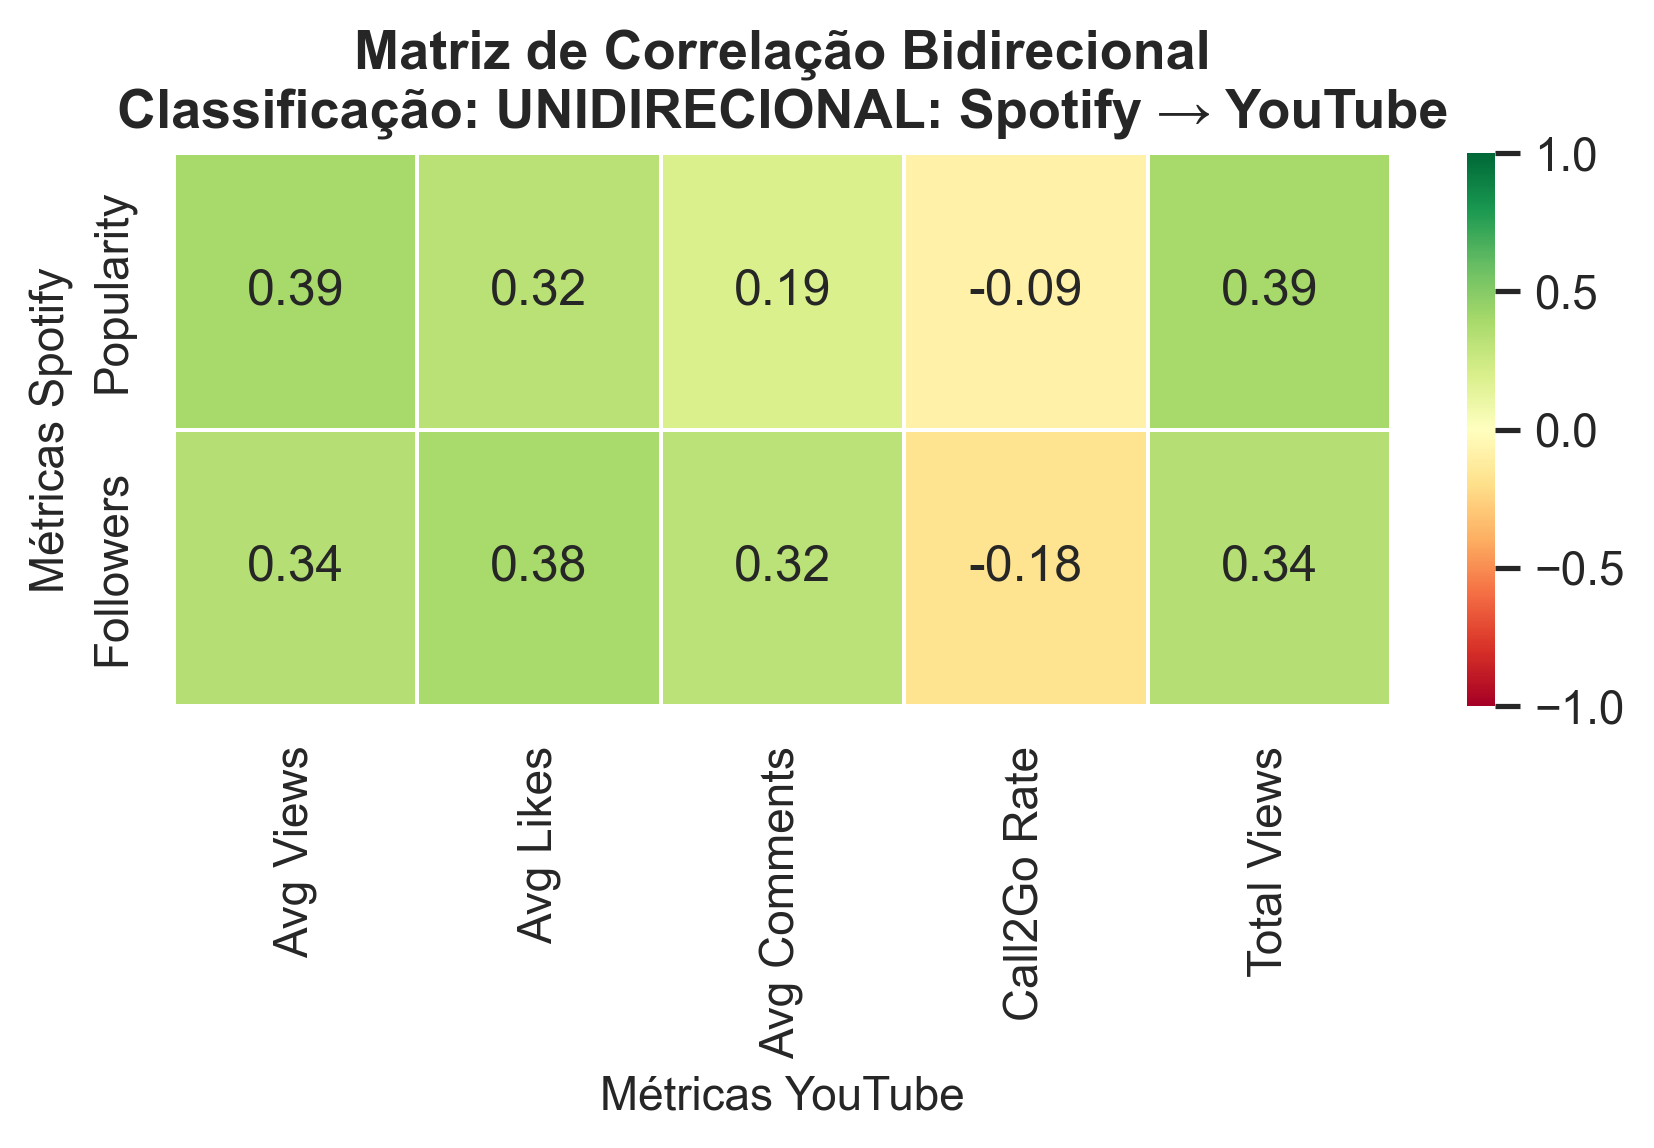
\includegraphics[width=0.85\textwidth]{../artigo_latex/figs/bidirectional_correlation_matrix.png}
\caption{Matriz de correlação bidirecional (Spearman) entre métricas YouTube
  e Spotify ($N = 67$ artistas). Cores quentes = correlação alta; cores frias
  = correlação baixa.}
\label{fig:heatmap}
\end{figure}

\subsection{O que é correlação de Spearman?}

\term{Correlação} mede o quanto duas variáveis ``andam juntas''. O coeficiente
$\rho$ (``rô'') de Spearman varia de $-1$ a $+1$:

\begin{itemize}
  \item $\rho = +1$: correlação perfeita positiva (quando um sobe, o outro
        sempre sobe junto).
  \item $\rho = 0$: sem correlação (os dois não têm relação).
  \item $\rho = -1$: correlação perfeita negativa (quando um sobe, o outro
        sempre desce).
\end{itemize}

\textbf{Por que Spearman (e não Pearson)?} O Spearman usa as \textbf{posições}
(rankings) dos valores em vez dos valores brutos. Isso é mais robusto quando
os dados têm distribuições muito assimétricas, que é justamente o caso de
visualizações do YouTube.

\subsection{Por que a análise foi ``bidirecional''?}

A análise foi feita nos dois sentidos para descobrir se a influência vai de
YouTube para Spotify, de Spotify para YouTube, ou dos dois lados:

\begin{itemize}
  \item \textbf{Direção A (YouTube $\to$ Spotify)}: A taxa de Call2Go de um
        artista no YouTube prevê a popularidade/seguidores dele no Spotify?
        (Ou seja: usar Call2Go faz crescer no Spotify?)
  \item \textbf{Direção B (Spotify $\to$ YouTube)}: A popularidade/seguidores
        de um artista no Spotify prevê as visualizações dele no YouTube? (Ou
        seja: quem é grande no Spotify também é grande no YouTube?)
\end{itemize}

\subsection{Resultados}

\medskip
\begin{center}
\begin{tabular}{llrrl}
\toprule
\textbf{Direção} & \textbf{O que foi correlacionado} & $\rho$ & $p$ &
  \textbf{Sig.} \\
\midrule
A: YT $\to$ SP & Taxa Call2Go $\leftrightarrow$ Popularidade Spotify
  & $0{,}008$ & $0{,}947$ & n.s. \\
A: YT $\to$ SP & Taxa Call2Go $\leftrightarrow$ Seguidores Spotify
  & $0{,}019$ & $0{,}877$ & n.s. \\
\midrule
B: SP $\to$ YT & Popularidade Spotify $\leftrightarrow$ Média views YT
  & $0{,}505$ & $<0{,}001$ & *** \\
B: SP $\to$ YT & Seguidores Spotify $\leftrightarrow$ Média views YT
  & $0{,}674$ & $<0{,}001$ & *** \\
\bottomrule
\end{tabular}
\end{center}
\medskip
\small\textit{n.s.\ = não significativo; *** = altamente significativo ($p <
0{,}001$); SP = Spotify; YT = YouTube}\normalsize

\bigskip
\textbf{Como ler cada linha:}

\begin{itemize}
  \item \textbf{Direção A, linha 1 ($\rho = 0{,}008$, $p = 0{,}947$)}: A taxa
        de Call2Go de um artista \textbf{praticamente não tem relação} com a
        popularidade dele no Spotify. Um $\rho$ de $0{,}008$ é
        indistinguível de zero. O $p = 0{,}947$ confirma: há 94,7\% de chance
        de essa correlação mínima ser puro acaso.

  \item \textbf{Direção A, linha 2 ($\rho = 0{,}019$, $p = 0{,}877$)}:
        Mesma conclusão para seguidores. Usar Call2Go no YouTube não prevê
        quantos seguidores o artista tem no Spotify.

  \item \textbf{Direção B, linha 1 ($\rho = 0{,}505$, $p < 0{,}001$)}:
        Artistas com mais popularidade no Spotify tendem a ter mais
        visualizações no YouTube. Um $\rho = 0{,}505$ é uma correlação
        \textbf{moderada a forte}. O $p < 0{,}001$ significa que há menos
        de 0,1\% de chance de ser acaso --- é uma relação real e confiável.

  \item \textbf{Direção B, linha 2 ($\rho = 0{,}674$, $p < 0{,}001$)}:
        Artistas com mais \textbf{seguidores} no Spotify têm muito mais
        visualizações no YouTube. Um $\rho = 0{,}674$ é uma correlação
        \textbf{forte}. A relação é mais clara ainda com seguidores do que com
        popularidade.
\end{itemize}

\textbf{Conclusão principal da análise bidirecional:} A influência vai de
\textbf{Spotify para YouTube}, e não o contrário. Quem é grande no Spotify
também é grande no YouTube. Mas usar Call2Go no YouTube \textbf{não garante}
crescimento no Spotify. A ``causalidade percebida'' é invertida: a estratégia
pode até ajudar individualmente, mas no conjunto dos 67 artistas não aparece
como fator determinante.

\textbf{O que o heatmap mostra (Figura~\ref{fig:heatmap}):} É uma grade
colorida onde cada célula representa a correlação entre duas variáveis. A
\textbf{parte de cima} da figura (Direção A) está em tons frios (azul):
correlações baixas, quase zero. A \textbf{parte de baixo} (Direção B) está
em tons quentes (laranja/vermelho): correlações altas. A assimetria visual
entre as duas metades é a conclusão principal do estudo bidirecional.

% ============================================================
\section{Análise temporal: o YouTube precede os charts}
% ============================================================

\begin{figure}[h!]
\centering
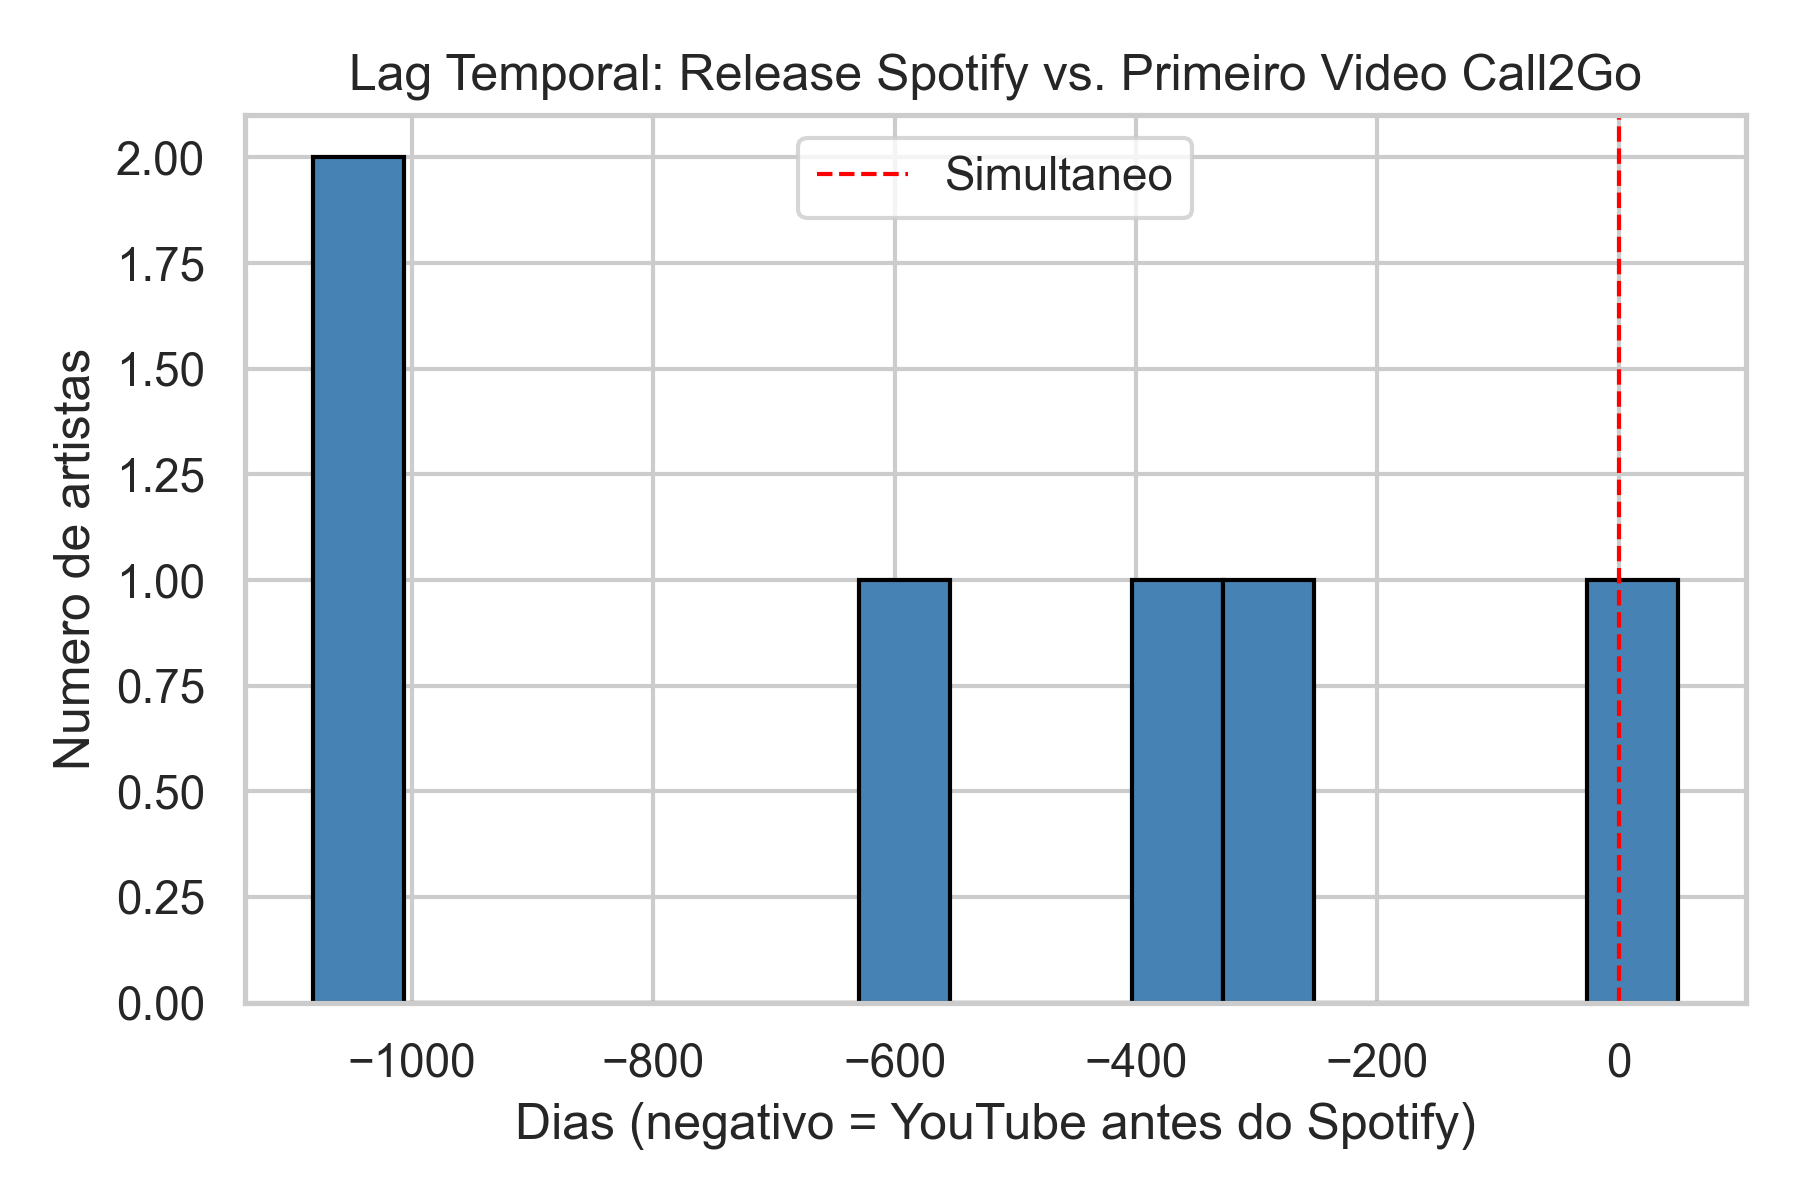
\includegraphics[width=0.90\textwidth]{../artigo_latex/figs/temporal_lag_analysis.png}
\caption{Defasagem temporal (dias) entre atividade no YouTube e entrada nos
  charts Spotify BR ($n = 39$ artistas). Valores negativos = YouTube veio
  antes dos charts.}
\label{fig:temporal}
\end{figure}

\subsection{O que é o ``lag'' (defasagem)?}

\term{Lag} é a \textbf{diferença em dias} entre dois eventos:

\begin{itemize}
  \item \textbf{Evento 1}: Data do primeiro vídeo publicado pelo artista no
        YouTube.
  \item \textbf{Evento 2}: Data em que o artista apareceu pela primeira vez
        no Top 200 Brasil do Spotify.
\end{itemize}

Se o lag é \textbf{negativo} (ex.: $-882$ dias), significa que o YouTube veio
\textbf{antes} dos charts --- o artista já publicava no YouTube quase 882 dias
antes de entrar nos charts do Spotify.

\subsection{Por que só 39 artistas?}

Dos 67 artistas, só foi possível calcular o lag para \num{39} porque:
\begin{itemize}
  \item Era preciso saber a data exata do primeiro vídeo no YouTube E a data
        de estreia nos charts do Spotify.
  \item Nem todos os artistas tinham dados históricos suficientes disponíveis
        nas APIs no momento da coleta.
\end{itemize}

\subsection{Resultados principais}

\begin{itemize}
  \item \textbf{Mediana de $-882$ dias}: Em metade dos 39 artistas, o YouTube
        veio pelo menos \num{882 dias} (cerca de \num{2,5 anos!}) antes de
        entrarem nos charts do Spotify. O YouTube é literalmente o palco onde
        a reputação é construída antes do sucesso nos charts.

  \item \textbf{IQR: $[-1.814;\; -360]$ dias}: O intervalo onde ficam os 50\%
        do meio dos artistas. Mesmo o extremo menor é $-360$ dias --- quase um
        ano de antecedência. E o extremo maior é $-1.814$ dias --- quase 5
        anos!

  \item \textbf{95\% dos artistas} tinham o YouTube precedendo os charts:
        apenas 2 artistas (5\%) tinham entrado nos charts antes de começar a
        publicar no YouTube.

  \item \textbf{18 artistas com Call2Go pré-chart}: dos 39, 18 usaram Call2Go
        \textbf{antes} de entrar nos charts. A mediana do lag de Call2Go desses
        18 foi de $-824$ dias. E \num{89\% (16 de 18)} deles adotaram a
        estratégia antes da estreia nos charts.
\end{itemize}

\subsection{Os preditores temporais (Tabela de correlações)}

Foram testadas 3 correlações para entender o que, na atividade do YouTube,
está relacionado com o desempenho posterior nos charts:

\medskip
\begin{center}
\begin{tabular}{lrrl}
\toprule
\textbf{O que foi testado} & $\rho$ & $p$ & \textbf{Sig.} \\
\midrule
Vídeos publicados nos 30 dias antes dos charts
  $\leftrightarrow$ Score combinado           & $0{,}364$ & $0{,}022$ & *   \\
Lag Call2Go (dias) $\leftrightarrow$ Score Spotify
                                              & $0{,}028$ & $0{,}913$ & n.s.\\
Call2Go presente pré-chart (sim/não)
  $\leftrightarrow$ Score Spotify             & $-0{,}093$ & $0{,}575$ & n.s.\\
\bottomrule
\end{tabular}
\end{center}
\medskip
\small\textit{* $p < 0{,}05$; n.s.\ = não significativo}\normalsize

\bigskip
\textbf{Como interpretar:}

\begin{itemize}
  \item \textbf{Linha 1 ($\rho = 0{,}364$, $p = 0{,}022$) --- o único
        preditor significativo}: Artistas que publicaram mais vídeos no
        YouTube nos \textbf{30 dias imediatamente antes} de entrar nos charts
        tendem a ter um score combinado melhor. $\rho = 0{,}364$ é uma
        correlação fraca a moderada, mas o $p = 0{,}022$ confirma que não é
        acaso. Faz sentido intuitivamente: mais conteúdo recente = mais
        visibilidade = mais momentum = melhor posicionamento inicial nos
        charts.

  \item \textbf{Linha 2 ($\rho = 0{,}028$, $p = 0{,}913$)}: O tempo de
        antecedência do Call2Go (quantos dias antes dos charts o artista
        começou a usar Call2Go) \textbf{não prevê} o score no Spotify.
        Adotar Call2Go mais cedo não garante mais popularidade.

  \item \textbf{Linha 3 ($\rho = -0{,}093$, $p = 0{,}575$)}: Ter ou não
        ter usado Call2Go antes de entrar nos charts não tem relação com a
        popularidade posterior no Spotify.
\end{itemize}

\textbf{O que o gráfico temporal mostra (Figura~\ref{fig:temporal}):} Cada
ponto é um artista. O eixo X é a defasagem em dias. A grande maioria dos
pontos está à esquerda de zero (YouTube veio antes dos charts). A linha
central (mediana) está em $-882$ dias, dividindo os artistas ao meio.

% ============================================================
\section{Last.fm e auditoria de voltas}
% ============================================================

\subsection{O que é o Last.fm nesse contexto?}

\term{Last.fm} é uma rede social de música que registra automaticamente o que
você ouve em qualquer player compatível. Cada reprodução registrada é chamada
de \term{scrobble}. Ela serve como \textbf{terceira plataforma independente}:
se um artista é realmente popular no Brasil, ele deveria aparecer no YouTube E
no Spotify E no Last.fm.

Dos 67 artistas, \num{9 (13,4\%)} estavam ao mesmo tempo no Top 200 Brasil do
Last.fm. Isso é esperado: o Last.fm tem base de usuários menor e mais
específica que Spotify e YouTube.

\subsection{Correlação Last.fm $\times$ Spotify}

\begin{itemize}
  \item \textbf{$\rho = 0{,}848$, $p < 0{,}001$}: Artistas com mais
        seguidores no Spotify têm significativamente mais scrobbles no Last.fm.
        Um $\rho = 0{,}848$ é uma correlação \textbf{muito forte} --- quase
        perfeita. Isso serve como \textbf{validação cruzada} dos dados:
        confirma que os dados do Spotify estão corretos e que os artistas
        analisados são de fato populares de forma consistente entre plataformas.
\end{itemize}

\subsection{Call2Go afeta métricas no Last.fm?}

\begin{itemize}
  \item \textbf{Listeners Last.fm: $p = 0{,}865$ (n.s.)}: artistas com Call2Go
        não têm mais ouvintes mensais no Last.fm.
  \item \textbf{Scrobbles Last.fm: $p = 0{,}960$ (n.s.)}: artistas com Call2Go
        não têm mais scrobbles registrados.
  \item \textbf{Presença nos charts Last.fm: $\chi^2 = 2{,}610$,
        $p = 0{,}106$ (n.s.)}: usar Call2Go não prevê aparecer nos charts do
        Last.fm.
  \item \textbf{Gênero musical: $\chi^2 = 2{,}293$, $p = 0{,}682$ (n.s.)}:
        o gênero musical do artista (sertanejo, funk, pop etc.) não influencia
        no uso de Call2Go.
\end{itemize}

\textbf{Resumo:} o Call2Go não tem relação com popularidade no Last.fm
também. A consistência de resultados nulos nas três plataformas fortalece a
conclusão do estudo.

\subsection{O que é a ``auditoria de voltas''?}

A auditoria verificou se algum artista criava um \textbf{ciclo bidirecional}:
link do YouTube apontando para Spotify (Call2Go) E link do Spotify/Last.fm
apontando de volta para o YouTube.

Resultado: \num{0 de 67 artistas} tinham links reversos em nenhuma das 4
direções verificadas. Ou seja, a estratégia é \textbf{estritamente
unidirecional}: YouTube leva para Spotify, mas Spotify não leva de volta para
YouTube.

% ============================================================
\section{A validação do detector}
% ============================================================

\begin{figure}[h!]
\centering
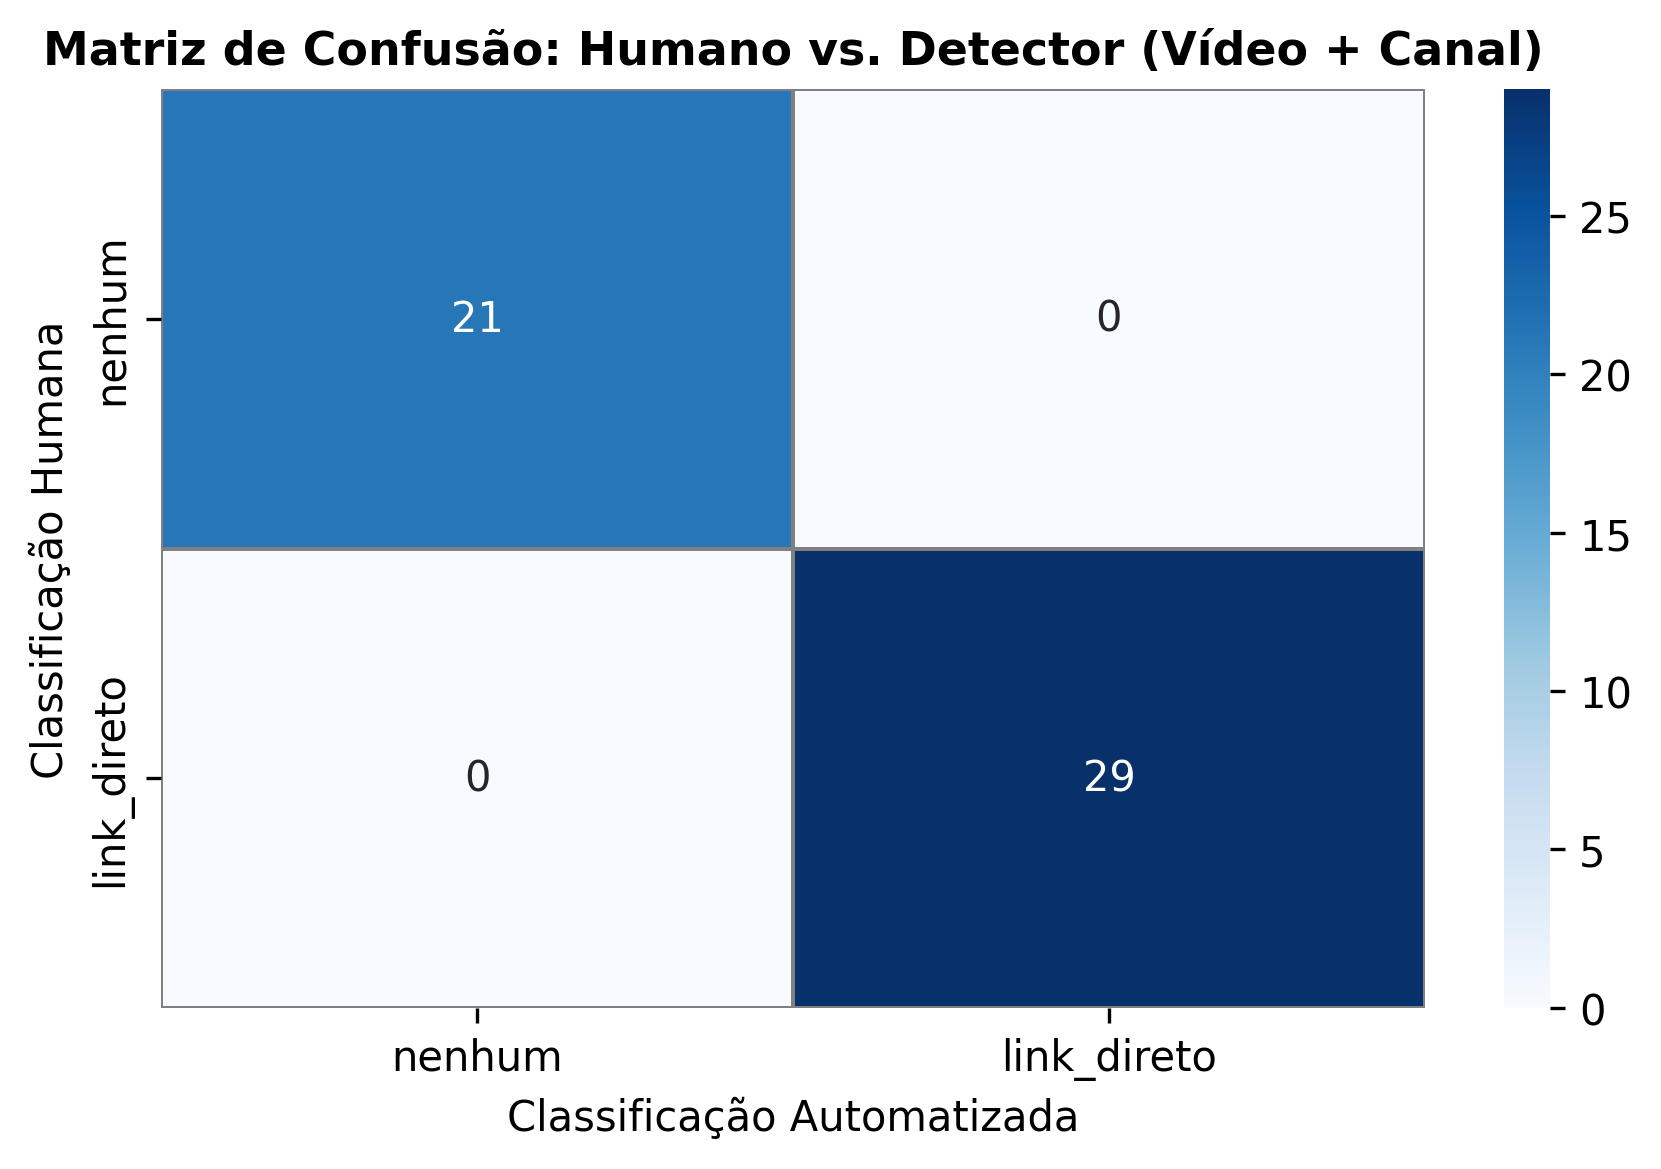
\includegraphics[width=0.85\textwidth]{../artigo_latex/figs/confusion_matrix_combined.png}
\caption{Matriz de confusão: comparação entre o detector automático e a
  classificação humana (91 vídeos adversariais, anotação às cegas).
  Esquerda: nível canal. Direita: nível vídeo.}
\label{fig:confusion}
\end{figure}

\subsection{O que é a validação cruzada do detector?}

Para saber se o detector está \textbf{acertando}, ele foi testado contra a
opinião de um humano. A metodologia foi:

\begin{enumerate}
  \item Selecionou-se \num{91 vídeos adversariais}: casos propositalmente
        difíceis de classificar (os mais ambíguos do corpus).
  \item Um anotador humano analisou cada vídeo \textbf{sem saber} o que o
        detector tinha classificado --- isso é chamado de \term{anotação às
        cegas}, e serve para evitar que o humano seja influenciado pela
        resposta do detector.
  \item As classificações do humano foram comparadas com as do detector.
\end{enumerate}

\subsection{O que é a Matriz de Confusão?}

A matriz de confusão (Figura~\ref{fig:confusion}) divide os resultados em 4
categorias:

\begin{itemize}
  \item \textbf{VP (Verdadeiro Positivo)}: detector disse
        ``\textit{tem Call2Go}'' e humano concordou. \ok{Acerto.}
  \item \textbf{VN (Verdadeiro Negativo)}: detector disse
        ``\textit{sem Call2Go}'' e humano concordou. \ok{Acerto.}
  \item \textbf{FP (Falso Positivo)}: detector disse
        ``\textit{tem Call2Go}'' mas humano discordou.
        \alerta{Erro: detector marcou algo que não era Call2Go.}
  \item \textbf{FN (Falso Negativo)}: detector disse
        ``\textit{sem Call2Go}'' mas humano disse que tinha.
        \alerta{Erro: detector perdeu um Call2Go real.}
\end{itemize}

A \textbf{acurácia} é simplesmente: (VP + VN) / total. Ou seja, a
porcentagem de vezes que o detector acertou.

\subsection{O que é o Kappa de Cohen ($\kappa$)?}

A acurácia simples pode enganar. Se o detector dissesse ``sem Call2Go'' para
\textbf{tudo}, acertaria 68,4\% das vezes --- porque 68,4\% dos vídeos
realmente não têm Call2Go! Seria uma acurácia alta, mas o detector seria
inútil.

O \term{Kappa de Cohen ($\kappa$)} desconta esse acerto esperado por
coincidência. Ele responde: \textit{``Quanto \textbf{melhor que o acaso} o
detector está acertando?''}

Escala de interpretação do $\kappa$ (Landis \& Koch, 1977):

\medskip
\begin{center}
\begin{tabular}{cl}
\toprule
$\kappa$ & Interpretação \\
\midrule
$< 0{,}20$        & Péssimo \\
$0{,}21$--$0{,}40$ & Fraco \\
$0{,}41$--$0{,}60$ & Moderado \\
$0{,}61$--$0{,}80$ & Substancial (bom) \\
$> 0{,}80$        & Quase perfeito \\
\bottomrule
\end{tabular}
\end{center}
\medskip

\subsection{Resultados da validação}

\medskip
\begin{center}
\begin{tabular}{lccll}
\toprule
\textbf{Nível} & \textbf{Acurácia} & $\kappa$ & \textbf{Interpretação} &
  \textbf{Passou?} \\
\midrule
Canal (bio/links) & 90,1\% & 0,80 & Substancial & \ok{Sim ($\geq$ 85\%)} \\
Vídeo (descrição) & 82,4\% & 0,45 & Moderado    & \alerta{Não ($<$ 85\%)} \\
\bottomrule
\end{tabular}
\end{center}
\medskip

\textbf{Como interpretar:}

\begin{itemize}
  \item \textbf{Nível Canal ($\kappa = 0{,}80$, acurácia = 90,1\%)}: O
        detector de canal \ok{passou no teste}. O limiar definido era de
        \num{85\%} de acurácia, e ele ficou em \num{90,1\%}. Um $\kappa$ de
        $0{,}80$ está no topo da faixa ``substancial'', quase na categoria
        ``quase perfeito''. Isso significa que o detector de canal é
        \textbf{confiável para uso em pesquisa}.

  \item \textbf{Nível Vídeo ($\kappa = 0{,}45$, acurácia = 82,4\%)}: O
        detector de vídeo \alerta{ficou 2,6 pontos percentuais abaixo do
        limiar} de 85\%. O $\kappa = 0{,}45$ é ``moderado'' --- funciona,
        mas com uma margem de erro maior. Casos onde só o vídeo (e não o
        canal) detectou Call2Go devem ser interpretados com mais cautela.

  \item \textbf{Por que a diferença entre os dois níveis?} A detecção no
        canal é mais fácil: os links na aba ``Sobre'' do YouTube são
        estruturados e bem formatados. A detecção no vídeo é mais difícil:
        a descrição é texto livre --- cada artista escreve de um jeito
        diferente, com abreviações, emojis e variações imprevisíveis.
\end{itemize}

% ============================================================
\section{O que concluímos? (H0 a H4 em linguagem direta)}
% ============================================================

O TCC testou 5 hipóteses. Aqui está o resultado de cada uma em linguagem
direta, sem fórmulas:

\medskip
\begin{description}[leftmargin=1.8em, style=nextline]

  \item[\textbf{H0/H1 --- O detector é confiável?}]
    \ok{Parcialmente sim.}\\
    O detector de \textbf{canal} é confiável (90,1\% de acurácia,
    $\kappa=0{,}80$) e passou no limiar definido. O detector de
    \textbf{vídeo} é razoável mas não chegou ao limiar (82,4\%,
    $\kappa=0{,}45$). Para análises futuras, o nível canal é o mais
    recomendado. O detector combinado (OR/AND) pode ser usado com a ciência
    de que o componente de vídeo tem maior margem de erro.

  \item[\textbf{H2 --- Call2Go aumenta visualizações no YouTube?}]
    \alerta{Não encontramos evidência.}\\
    $p = 0{,}872$ (OR). Vídeos com e sem Call2Go têm praticamente as mesmas
    visualizações. Colocar o link do Spotify na descrição não está se
    traduzindo em mais views.

  \item[\textbf{H3 --- Call2Go aumenta popularidade no Spotify?}]
    \alerta{Não encontramos evidência.}\\
    $p = 1{,}000$ (OR). Artistas com mais Call2Go têm a mesma popularidade
    no Spotify que artistas sem Call2Go. O $p = 1{,}000$ é o valor mais
    extremo possível de ``sem diferença alguma''.

  \item[\textbf{H4 --- A atividade no YouTube precede a entrada nos charts
    Spotify?}]
    \ok{Sim, e de forma muito expressiva.}\\
    Em 95\% dos artistas, o YouTube veio antes dos charts. A mediana foi de
    882 dias (mais de 2 anos) de antecedência. O único preditor
    estatisticamente significativo foi o volume de publicações nos 30 dias
    antes da estreia nos charts ($\rho = 0{,}364$, $p = 0{,}022$): quem
    publicou mais perto da estreia performou melhor nos charts.

  \item[\textbf{Correlação bidirecional (adicional)}]
    \ok{Spotify influencia YouTube, não o contrário.}\\
    A fama no Spotify prevê as visualizações no YouTube ($\rho = 0{,}674$),
    mas usar Call2Go no YouTube não prevê nada no Spotify ($\rho = 0{,}008$).
    O sentido da influência é Spotify $\to$ YouTube, não YouTube $\to$
    Spotify.

\end{description}

\textbf{Grande conclusão do TCC em uma frase:} Encontramos que o YouTube é
usado como palco de construção de audiência \textbf{muito antes} do sucesso no
Spotify, mas a estratégia de Call2Go, apesar de amplamente adotada (31,6\%
dos vídeos), não mostra impacto estatístico mensurável nas métricas de
engajamento.

% ============================================================
\section{Glossário rápido}
% ============================================================

\begin{description}[leftmargin=1.8em]

  \item[\term{API}] Interface que permite que um programa acesse dados de
        outro sistema de forma automática. Ex.: a API do Spotify permite
        consultar popularidade e seguidores de qualquer artista via código
        Python.

  \item[\term{Bootstrap (IC 95\%)}] Técnica estatística que repete a análise
        \num{10.000 vezes} com amostras ligeiramente diferentes para calcular
        intervalos de confiança sem precisar assumir que os dados têm
        distribuição normal.

  \item[\term{Call2Go}] Chamada de ação num vídeo do YouTube que direciona o
        ouvinte para o Spotify.

  \item[\term{Chart}] Ranking das músicas ou artistas mais ouvidos/vistos numa
        plataforma. Ex.: Spotify Top 200 Brasil, YouTube Top 100 Brasil.

  \item[\term{Cross-platform}] Que envolve mais de uma plataforma digital ao
        mesmo tempo. Aqui: YouTube + Spotify + Last.fm.

  \item[\term{EDA (Exploratory Data Analysis)}] Análise exploratória de dados:
        a etapa de ``olhar os dados'' antes de qualquer teste formal, usando
        gráficos e estatísticas descritivas.

  \item[\term{Kappa de Cohen ($\kappa$)}] Medida de concordância entre dois
        classificadores que desconta a concordância esperada por acaso. Vai de
        0 (puro acaso) a 1 (concordância perfeita).

  \item[\term{Lag (defasagem)}] Diferença em dias entre dois eventos temporais.
        Aqui: dias entre o primeiro vídeo no YouTube e a estreia nos charts do
        Spotify.

  \item[\term{Mann-Whitney U}] Teste estatístico para comparar dois grupos sem
        assumir que os dados seguem distribuição normal.

  \item[\term{Pipeline ETL}] Sequência automatizada de passos:
        \textbf{E}xtração de dados, \textbf{T}ransformação e \textbf{L}arga
        (\textit{Extract, Transform, Load}).

  \item[\term{Regex (expressão regular)}] Sistema de busca de padrões em texto
        usando regras formais. É como um Ctrl+F avançado que entende variações,
        proximidade e contexto.

  \item[\term{Scraping}] Técnica de coleta automática de dados de páginas web
        que não têm API disponível. O programa lê o HTML da página e extrai
        as informações de interesse.

  \item[\term{Scrobble (Last.fm)}] Registro de uma música ouvida na plataforma
        Last.fm. Cada vez que você reproduz uma música, um ``scrobble'' é
        adicionado ao seu perfil.

  \item[\term{Spearman ($\rho$)}] Coeficiente de correlação que usa posições
        (rankings) em vez de valores brutos. Vai de $-1$ a $+1$.

  \item[\term{Star schema}] Modelo de banco de dados com uma tabela central de
        fatos (os dados principais) e tabelas de dimensão ao redor. É o modelo
        padrão para bancos de dados voltados a análises.

  \item[\term{Valor-p ($p$-value)}] Probabilidade de observar o resultado
        obtido \textbf{por acaso}, assumindo que não existe efeito real.
        $p < 0{,}05$ = resultado significativo (difícil de ser acaso);
        $p \geq 0{,}05$ = sem evidência de efeito.

\end{description}

\vspace{3em}
\hrule
\vspace{0.8em}
\begin{center}
\small\textcolor{cinza}{\itshape
  Colinha criada em 29/04/2026 para alinhamento com orientador.\\
  Para uso exclusivo do autor.\\[0.3em]
  Todos os dados são provenientes do pipeline TCC Call2Go (commit
  \texttt{0bdfcf7}).
}
\end{center}

\end{document}
